\section{Levers for Offsetting Cost}

\subsection{Distribution as a Load-Side Lever}
\label{sec:load_side_lever}

\begin{figure}[t]
  \centering


    \begin{subfigure}[t]{\columnwidth}
    \centering
    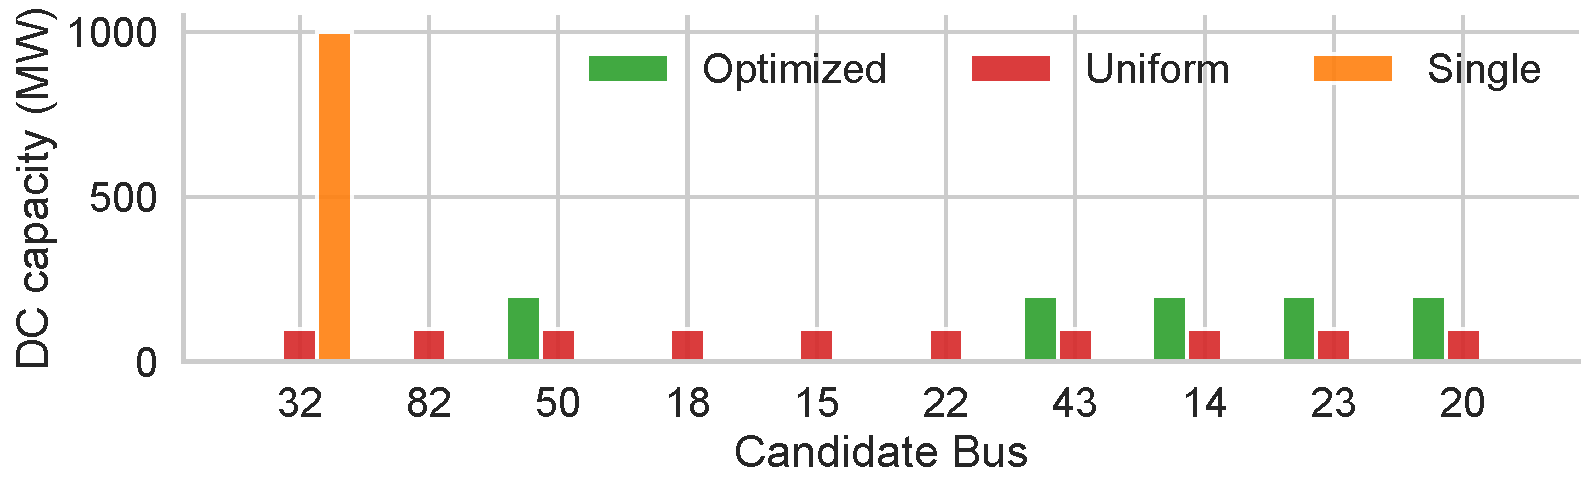
\includegraphics[width=\textwidth]{figures/dc_allocation_bar_plot-1.pdf}
    \caption{Planned data center capacity across candidate buses under different allocation policies.}
    \label{fig:dc_allocation_bar_plot}
  \end{subfigure}

  \begin{subfigure}[t]{\columnwidth}
    \centering
    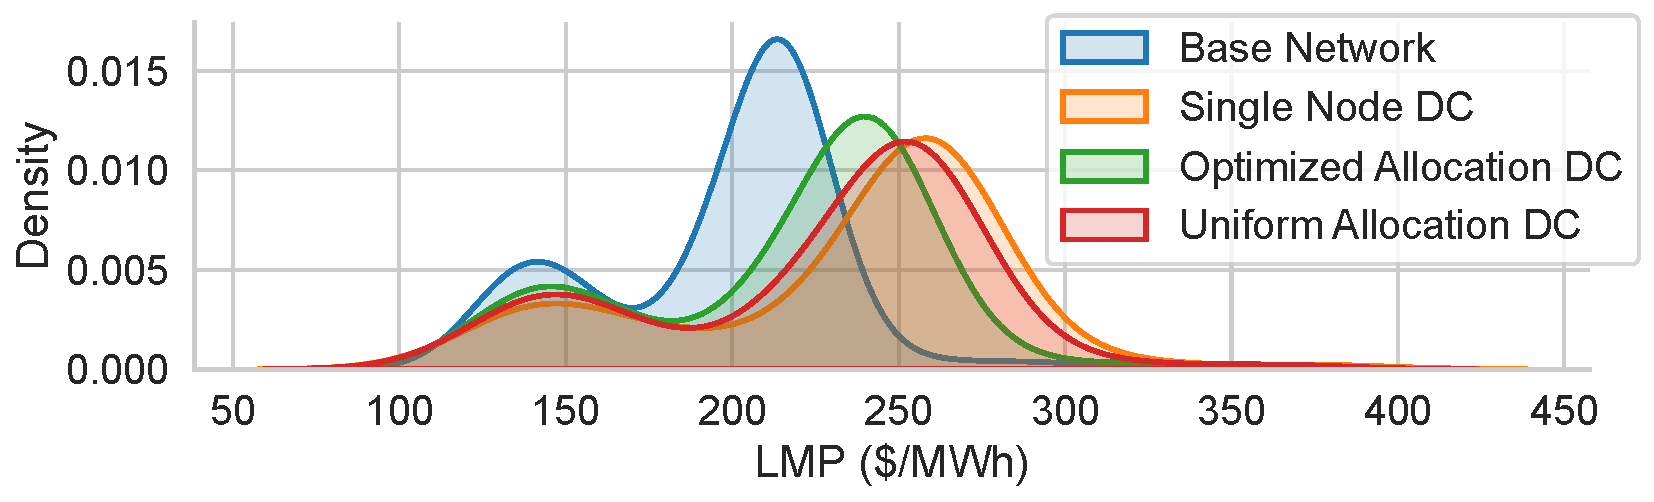
\includegraphics[width=\columnwidth]{figures/kde_p95_lmp-1.pdf}
    \caption{P95 of LMP across buses.}
    \label{fig:kde_p95_lmp}
  \end{subfigure}
  
  \vspace{0.6em}

  \caption{System LMP shifts risk and data center capacity allocation.}
  \label{fig:lmp_and_allocation}
\end{figure}

We first examine the impacts of distributing datacenter capacity as a load-side lever to manage grid impacts. To understand the base dispatch, we solve Problem (\ref{eq:dc-opf-full}) with no datacenter load added to the system. For the single node injection case, we build a single 1GW datacenter at the cheapest land cost node from the set of candidate buses selected according to the methodology in Section \ref{sec:candidate_selection}. To determine the optimized distributed allocation, we first fix $K=10$ buses from the candidate set. The minimum and maximum allowable datacenter capacities at each location are set to $\underline{\eta}=50$MW and $\overline{\eta}=250$MW respectively.  All candidate nodes utilize the inference workload profile. We then solve Problem (\ref{eq:dc_plan}) with 10 steps of projected gradient descent with $\alpha=20$, $\beta=1000$, and step size $s=0.01$. To determine the uniform allocation, we assign 100MW of capacity to each of the 10 nodes. In all cases where we provision datacenter capacity, we solve Problem (\ref{eq:dc-opf-full}) with the determined capacities at each of the specified buses to examine the LMPs and flows in the system. 

Figure \ref{fig:dc_allocation_bar_plot} shows the single node, uniform, and optimized allocations. The optimized allocation selects only a subset of the candidate nodes at which to allocate 200MW each. For each scenario, we compute the $95\textsuperscript{th}$ percentile LMP at each node over the 24 hour simulation window. Figure \ref{fig:kde_p95_lmp} shows the kernel density estimates for the spatial distribution of P95 LMPs at each bus. We observe that the optimized allocation pushes the P95 prices lower towards the base dispatch prices. Naive distribution as is done in the uniform case does not show substantial improvement over the single node injection. While not shown, we note that the distributions look similar when the temporal aggregation metric at each node is max or mean instead of the $95\textsuperscript{th}$ percentile. 

\subsection{Comparative Analysis of Levers}

We compare several expansion scenarios to assess how distributed datacenter placement performs relative to conventional grid-side levers. The single node and optimized distributed datacenter allocations are determined according to the methods in Section~\ref{sec:load_side_lever}. We then consider the same single node injection of 1~GW, but allow for either transmission or generation expansion. Finally, we consider the optimized distributed allocation with either transmission or generation expansion to demonstrate the combined effects of multiple levers.

For transmission expansion, we solve Problem~\eqref{eq:trans_plan} with $\mathcal{E} = \mathcal{E}_{\text{trans}}$ using 10 steps of projected gradient descent with step size $s = 0.01$, allowing up to a 5\% increase in transmission capacity per line. For generation expansion, we solve the analogous problem with $\mathcal{E} = \mathcal{E}_{\text{gen}}$, allowing up to a 2.5\% increase in capacity per generator. In both cases, the planning objective is $\gamma^\top \eta + h_{\text{dispatch}}$, reflecting that these are system upgrades where the grid operator seeks to minimize investment while reducing operational cost.

For combined scenarios, we first solve Problem~\eqref{eq:dc_plan} to determine the distributed datacenter allocation, then subsequently solve the transmission or generation expansion problem with the distributed capacity injected into the network. We optimize these sequentially rather than jointly due to the discrepancy in planning objectives. Transmission and generation are system upgrades planned to minimize investment and dispatch cost, whereas datacenter placement is not a system upgrade and may prioritize factors like LMPs that fall outside standard grid operator objectives. This separation also reflects realistic institutional constraints, where datacenter operators select sites based on their own objectives before grid operators plan responsive upgrades.

\paragraph{Metrics.}
For each scenario, we report annualized investment cost (M\$/yr) over a 20-year horizon with a 7\% discount rate, and dispatch cost (M\$/day) for the simulated day of operation. Given the matrix of nodal LMPs $\Lambda \in \mathbb{R}^{N \times T}$, we compute the following LMP metric: 
% {\setlength{\abovedisplayskip}{3pt}
%  \setlength{\belowdisplayskip}{3pt}
\begin{equation}
\mathrm{LMP} = \frac{1}{N}\sum_{n=1}^{N}\max_{t\in\{1,\dots,T\}} \Lambda_{n,t}.
\end{equation}
% }\noindent
which denotes the mean across nodes of the max LMP at each node over time. This serves as an interpretable proxy for the smooth-max objective used in optimization. To quantify congestion, we consider the shadow prices $\mu_\ell^+, \mu_\ell^-$ associated with the upper and lower transmission line flow constraints for each line $\ell$. At any timestep, at most one of these can be nonzero, so their sum captures the binding shadow price. We aggregate this as
\begin{equation}
    C = \frac{1}{L} \sum_{\ell=1}^{L} \max_{t \in \{1,\ldots,T\}} \left( \mu_\ell^+(t) + \mu_\ell^-(t) \right),
\end{equation}
which represents the average across lines of the peak shadow price over time. Table~\ref{tab:synopsis_tradeoffs_singlecol_ops} reports percentage change in this metric relative to the base scenario (no datacenter load).

\paragraph{Results.}
The results are summarized in Table~\ref{tab:synopsis_tradeoffs_singlecol_ops}. Distributing datacenter capacity across multiple sites reduces the LMP metric from 378.4~\$/MWh (single node) to 217.2~\$/MWh, yielding a 42.6\% reduction at nearly identical datacenter investment cost (1.21 vs.\ 1.19~M\$/yr). This LMP reduction is comparable to what is achieved by single-node injection paired with transmission expansion (216.6~\$/MWh), which requires 8$\times$ higher total investment (9.64~M\$/yr). Distribution also improves the congestion metric, reducing it from 24.66\% above base to 19.18\% above base.

Conventional grid-side levers, such as transmission and generation expansion, achieve similar LMP improvements but at substantially higher cost. Adding transmission capacity under single-node injection reduces congestion below the base scenario ($-4.11$\%), indicating that targeted upgrades can relieve pre-existing bottlenecks beyond offsetting the new load. Generation expansion reduces LMPs but is less effective at relieving congestion (14.38\% above base), consistent with the fact that added generation capacity does not directly alleviate transmission constraints.

The combined scenarios demonstrate that distribution and grid-side levers are complementary. Distributed placement paired with transmission expansion achieves the lowest LMP (202.4~\$/MWh) and congestion ($-7.08$\%) outcomes at similar cost to the single-node-plus-transmission case. This suggests that distributed siting improves the price response of the grid, allowing the same grid investment to go further. Notably, the transmission and generation expansions are modest relative to the datacenter load, adding 466--469~MW and 342--343~MW respectively against a 1~GW interconnection, yet yield meaningful improvements when combined with optimized placement.

Dispatch cost remains nearly constant across all scenarios (0.226--0.227~M\$/day). This is consistent with the observation that LMPs reflect local prices at constrained nodes, while dispatch cost captures total system operating cost. Congestion-induced redispatch affects prices at the margin, but if the volume of redispatched energy is small relative to total system load, aggregate dispatch cost may not shift substantially even as localized price spikes occur.

% To assess the efficacy of distributing provisioned datacenter capacity as a load-side lever relative to more conventional planning levers such as transmission and generation expansion, we run several expansion planning experiments and observe their impacts on various metrics. The single node and distributed datacenter allocation scenarios are determined according to the methods outlined in Section \ref{sec:load_side_lever}. We then consider the same single node injection of 1GW at a single site, but allow for either transmission or generation expansion as well. Finally, we consider the optimized distributed allocation of datacenter capacity and allow for either transmission or generation expansion to demonstrate the combined effects of using multiple levers in conjunction with each other. 

% In the single node datacenter case mitigated with transmission expansion, we solve Problem (\ref{eq:trans_exp}) using 10 steps of projected gradient descent with a step size of $s=0.01$. We allow for up to a $5\%$ increase in the transmission capacity of each line in the system. Similarly, for the single node case with generation expansion, we solve Problem (\ref{eq:gen_exp}) with the exact same algorithm parameters but allowing for up to $2.5\%$ increase in the capacity of each generator. 

% For the combined cases of distributed allocation in addition to transmission or generation expansion, we independently solve Problem (\ref{eq:dc_plan}) (as outlined in Section \ref{sec:load_side_lever}), and then subsequently solve either Problem (\ref{eq:trans_exp}) or (\ref{eq:gen_exp}) as specified above with the distributed capacity injected into the network. We choose \emph{not} to optimize datacenter capacity jointly with transmission or generation due to the discrepancy in planning objectives. The planning objective for transmission and generation expansion is $\gamma^{\top}\eta + h_{\text{dispatch}}$, while the datacenter expansion objective is only $h_{\text{LMP}}$. The transmission and generation expansion planning objectives reflect that these are \emph{system} upgrades in response to a large-load interconnection. While these upgrades may have been triggered by the load, the objective for the grid operator is to simultaneously minimize investment while reducing operational (dispatch) cost of the system. On the other hand, planning for datacenter capacity expansion is not a system upgrade, and thus there are various operational factors that may be important (like LMPs) that are outside the purview of standard grid operator objectives. 

% The results are summarized in Table \ref{tab:synopsis_tradeoffs_singlecol_ops}. For each scenario, we report the total investment cost (i.e. the sum of generation, transmission, and datacenter costs) as an annualized cost in M\$\slash yr. The dispatch cost for the 24 hour simulation window is also reported in M\$ \slash yr. Given the matrix of nodal LMPs $\Lambda \in \mathbb{R}^{N \times T}$, we compute the Table \ref{tab:synopsis_tradeoffs_singlecol_ops} metric ``LMP'' as 
% {\setlength{\abovedisplayskip}{3pt}
%  \setlength{\belowdisplayskip}{3pt}
% \begin{equation}
% \mathrm{LMP} = \frac{1}{N}\sum_{n=1}^{N}\max_{t\in\{1,\dots,T\}} \Lambda_{n,t}.
% \end{equation}}\noindent
% which denotes the mean across nodes of the max LMP at each node over time. 

% - explain the LMP metric
% - LMP result (distribution helps)
% - other levers help a similar amount but are way more expensive
% - in the combined case, distribution helps to push the LMPs down much more for a similar cost as to just transmission or generation. 

% - write down transmission line flow constraints
% - define the duals of mu+ and mu- of the transmission line flow constraints
% - define how we use those to form the congestion metric 
% - given an interpretation of the metric
% - explain that all results are reported relative to base (which is 0)
% - congestion result (distribution helps)
% - other levers help as well, and actually more. 
% - explain why this makes sense in the case of transmission expansion
% - explain how the combined case seems to help even more than just individual


% - note that dispatch cost doesn't seem to be changing much
% - explain why dispatch cost is not changing much 


\begin{table}[t]
\centering
\renewcommand{\arraystretch}{1.15}
\caption{Synopsis of planning tradeoffs across siting scenarios. Total investment cost (M\$/yr) are annualized over a 20yr period with a 7\% discount rate and dispatch costs (M\$/day) are calculated for the day of operation. LMPs are in \$\slash MWh. Congestion is \% change from the base scenario. }
\label{tab:synopsis_tradeoffs_singlecol_ops}
\resizebox{\columnwidth}{!}{
\begin{threeparttable}

\begin{tabular}{lccccccc}
\toprule
\textbf{Scenario} &
\textbf{Gen.} &
\textbf{Tx.} &
\textbf{DC} &
\textbf{Total} &
\textbf{LMP} &
\textbf{Dispatch} &
\textbf{Rel. Congestion} \\
\midrule
Base Case        & ---   & ---   & ---  & ---  & 196.78 & 0.225 & 0 \\
Single node (SN)        & ---   & ---   & 1.19 & 1.19 & 378.4 & 0.227 & 24.66 \\
Distributed (Dist)      & ---   & ---   & 1.21 & 1.21 & 217.2 & 0.227 & 19.18 \\
SN + transmission       & ---   & 8.45  & 1.19 & 9.64 & 216.6 & 0.227 & -4.11 \\
SN + generation         & 18.98 & ---   & 1.19 & 20.17 & 215.7 & 0.226 & 14.38 \\
Dist + transmission     & ---   & 8.48  & 1.21 & 9.69 & 202.4 & 0.226 & -7.08 \\
Dist + generation       & 19.18 & ---   & 1.21 & 20.38 & 205.0 & 0.226 & 8.22 \\
\bottomrule
\end{tabular}

\begin{tablenotes}[flushleft]\footnotesize
\item \textit{Notes:} ``+ transmission'' allows transmission expansion up to 5\% (added 466--469\,MW). ``+ generation'' allows generation expansion up to 2.5\% (added 342--343\,MW).
\end{tablenotes}
\end{threeparttable}
}
\end{table}


\section{Budget and Site Count Constraints}


\section{Workload Impacts on Placement}






